\documentclass[conference]{IEEEtran}
\IEEEoverridecommandlockouts
% The preceding line is only needed to identify funding in the first footnote. If that is unneeded, please comment it out.
%Template version as of 6/27/2024

\usepackage{cite}
\usepackage{amsmath,amssymb,amsfonts}
\usepackage{algorithmic}
\usepackage{graphicx}
\usepackage{textcomp}
\usepackage{xcolor}
\usepackage[colorlinks=true, allcolors=blue]{hyperref}
\usepackage{subcaption}
\usepackage{fontspec}

\pagestyle{plain}

\def\BibTeX{{\rm B\kern-.05em{\sc i\kern-.025em b}\kern-.08em
    T\kern-.1667em\lower.7ex\hbox{E}\kern-.125emX}}
\begin{document}

\title{An NDN-Based DNS Protocol for Improved Security and Efficiency in Edge Devices*\\
{\footnotesize \textsuperscript{*}Note: Sub-titles are not captured for https://ieeexplore.ieee.org and
should not be used}
\thanks{Identify applicable funding agency here. If none, delete this.}
}

\author{\IEEEauthorblockN{1\textsuperscript{st} Sameer G Kulkarni}
\IEEEauthorblockA{\textit{Computer Science and Engineering (Asst. Prof.)} \\
\textit{Indian Institute of Technology Gandhinagar}\\
Gandhinagar, India \\
sameergk@iitgn.ac.in}
\and
\IEEEauthorblockN{2\textsuperscript{nd} Mithil Pechimuthu}
\IEEEauthorblockA{\textit{Computer Science and Engineering (Student)} \\
\textit{Indian Institute of Technology Gandhinagar}\\
Gandhinagar, India \\
pechimuthumithil@iitgn.ac.in}
\and
\IEEEauthorblockN{3\textsuperscript{rd} Sachin Jalan}
\IEEEauthorblockA{\textit{Computer Science and Engineering (Student)} \\
\textit{Indian Institute of Technology Gandhinagar}\\
Gandhinagar, India \\
jalansachin@iitgn.ac.in}
\and
\IEEEauthorblockN{4\textsuperscript{th} Tirth Patel}
\IEEEauthorblockA{\textit{Computer Science and Engineering (Student)} \\
\textit{Indian Institute of Technology Gandhinagar}\\
Gandhinagar, India \\
pateltirth@iitgn.ac.in}
% \and
% \IEEEauthorblockN{5\textsuperscript{th} Given Name Surname}
% \IEEEauthorblockA{\textit{dept. name of organization (of Aff.)} \\
% \textit{name of organization (of Aff.)}\\
% City, Country \\
% email address or ORCID}
% \and
% \IEEEauthorblockN{6\textsuperscript{th} Given Name Surname}
% \IEEEauthorblockA{\textit{dept. name of organization (of Aff.)} \\
% \textit{name of organization (of Aff.)}\\
% City, Country \\
% email address or ORCID}
}

\maketitle

\begin{abstract}
The Domain Name System (DNS) protocol has remained unchanged since its inception in 1983. While it is efficient for general computing, the increasing importance and number of edge devices and IoT may reveal that the current DNS protocol implementation can be power-hungry, slow, and insecure. Experiments showed that the DNS protocol and its implementation have inefficiencies that cause overheads in resource-constrained environments, such as IoT devices with limited energy budgets. We motivate the need for a new DNS protocol and state the aspects that can be improved upon. The details of the experiments conducted are also present in this document. Finally, we propose a new DNS protocol based on Named Data Networking (NDN) that addresses security and efficiency issues while having a low power footprint. We used the ICARUS-ICN simulator to verify these claims; the results are presented in this document.
\end{abstract}

\begin{IEEEkeywords}
DNS, NDN, Security, Efficiency, Edge Devices, IoT
\end{IEEEkeywords}

\section{Introduction}
\subsection{Background on DNS}
The Domain Name System (DNS) is a hierarchical and decentralized naming system that serves as the backbone of modern Internet communication. It translates human-readable domain names, such as \texttt{www.example.com}, into machine-readable numerical IP addresses, enabling devices to locate and communicate with one another over the Internet. This process is crucial for the functionality of websites, email services, and numerous other online applications \cite{mockapetris1983dns}.

DNS was introduced in 1983 to address the challenges posed by maintaining a centralized host file for mapping domain names to IP addresses. Despite its robustness and scalability, the DNS protocol has largely remained unchanged since its inception. This legacy design leaves DNS vulnerable to various security threats, such as cache poisoning, spoofing, and distributed denial-of-service (DDoS) attacks. For example, let's say we want to resolve the domain name like "iitgn.ac.in," into IP addresses like 72.1.241.188, that machines use to address each other. Usually, all of the DNS operates using a recursive query mechanism, where a DNS resolver iteratively queries multiple DNS servers to resolve a domain name, starting from the root servers (contain info about .com, in, etc...) through the top-level domain (TLD) servers (provide .com, .in,  etc...), and down to the authoritative servers. Figure \ref{fig:dns-overview} shows the exact steps taken to resolve our example domain "iitgn.ac.in". 

\begin{figure}[htbp]
    \centering
    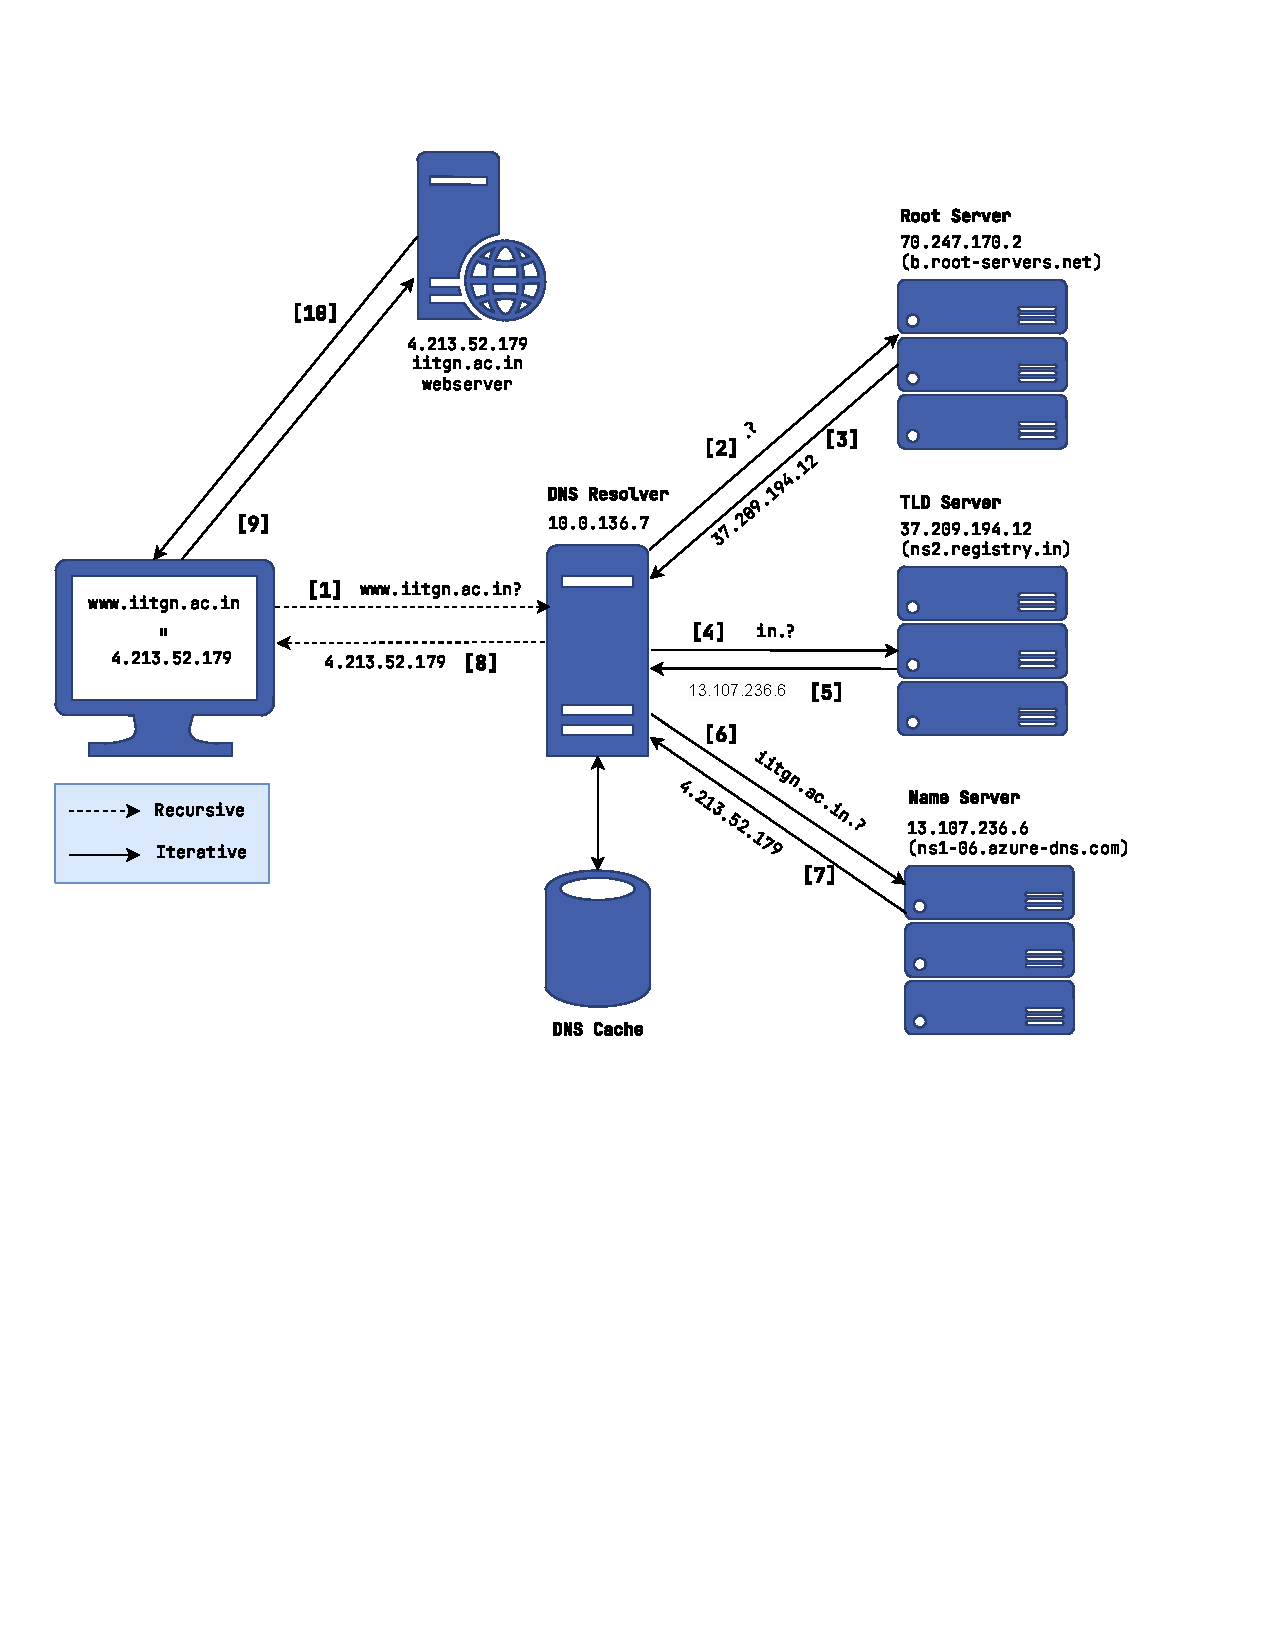
\includegraphics[width=1\linewidth,trim={0 10cm 0 2cm},clip]{images/dns-overview.pdf}
    \caption{DNS Architecture}
    \label{fig:dns-overview}
\end{figure}

\subsection{Integrating Security: DNS-SEC}
To mitigate these vulnerabilities, DNS Security Extensions (DNS-SEC) were introduced to enhance the protocol with mechanisms like digital signatures for DNS records. Figure \ref{fig:DNS-SEC-overview} represents the steps involved in DNS-SEC. 

\begin{figure}[htbp]
    \centering
    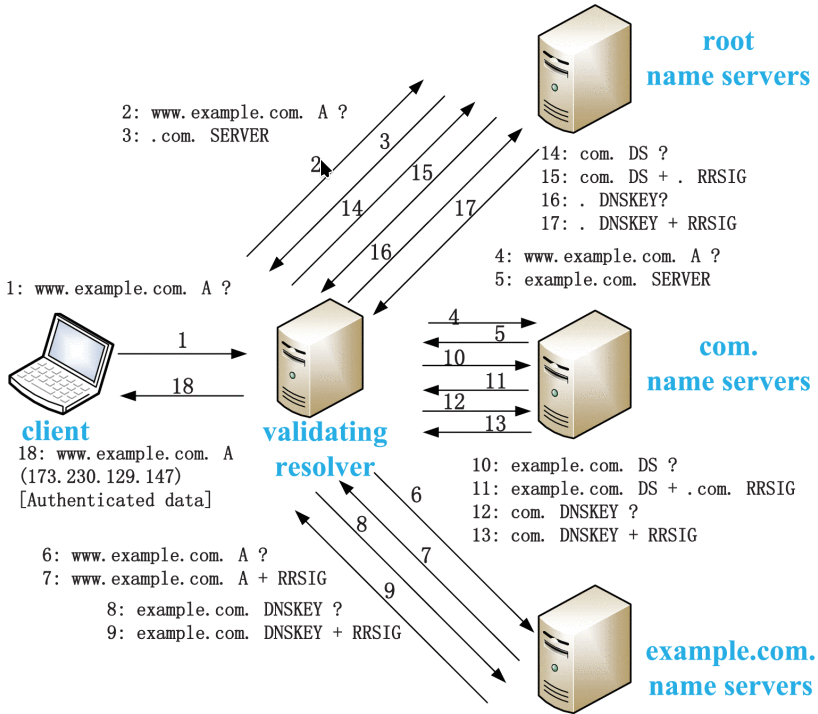
\includegraphics[width=1\linewidth]{images/dnssec-overview.png}
    \caption{DNS-SEC Architecture \cite{8653281}}
    \label{fig:DNS-SEC-overview}
\end{figure}

On comparing figures \ref{fig:dns-overview} and \ref{fig:DNS-SEC-overview} we can see that while DNS-SEC improves the security of DNS, it is complex and has high computational overhead \cite{8653281}. In addition to this overhead, implementation of DNS-SEC requires huge time and human resources and lack of global consensus \cite{polo-2022} prevent widespread adoption of DNS-SEC. This overhead is particularly problematic for resource-constrained devices, such as those used in IoT environments, which may lack the processing power or battery capacity to handle the added burden. The cryptographic operations involved in DNS-SEC, such as signature verification, are resource-intensive and can quickly deplete the limited battery life of edge devices. Figures \ref{fig:dns-cycles} and \ref{fig:dns-energy} show the resource consumed for plain DNS resolution. This only increases when complex protocols such as DNS-SEC is used. Additionally, the added latency from DNS-SEC validation may impact time-sensitive applications, such as real-time monitoring and control systems. Furthermore, frequent DNS lookups increase network overhead, which is particularly burdensome for low-power wide-area networks (LPWANs) that are commonly used in IoT deployments. These inefficiencies underline the need for alternative approaches or optimizations to make DNS suitable for edge environments. The section \ref{Measuring Protocol Inefficiencies} explains how we examine the DNS protocol and encountered some pain points.

\begin{figure}[htbp]
    \centering
    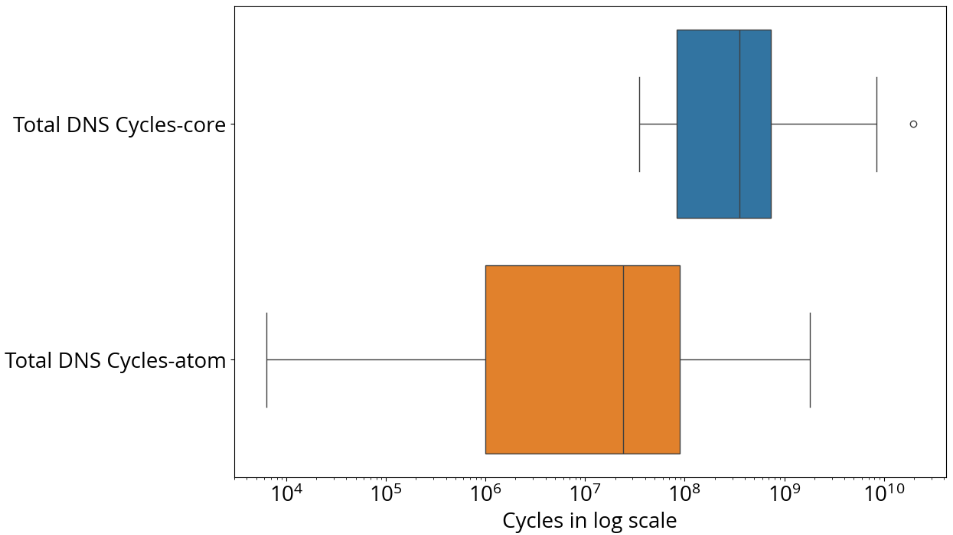
\includegraphics[width=1\linewidth]{images/cycles.png}
    \caption{This box plot shows the cycles (in log scale) consumed in the DNS resolution of every domain required to load a page, for the 1000 websites we tested.}
    \label{fig:dns-cycles}
\end{figure}
\begin{figure}[htbp]
    \centering
    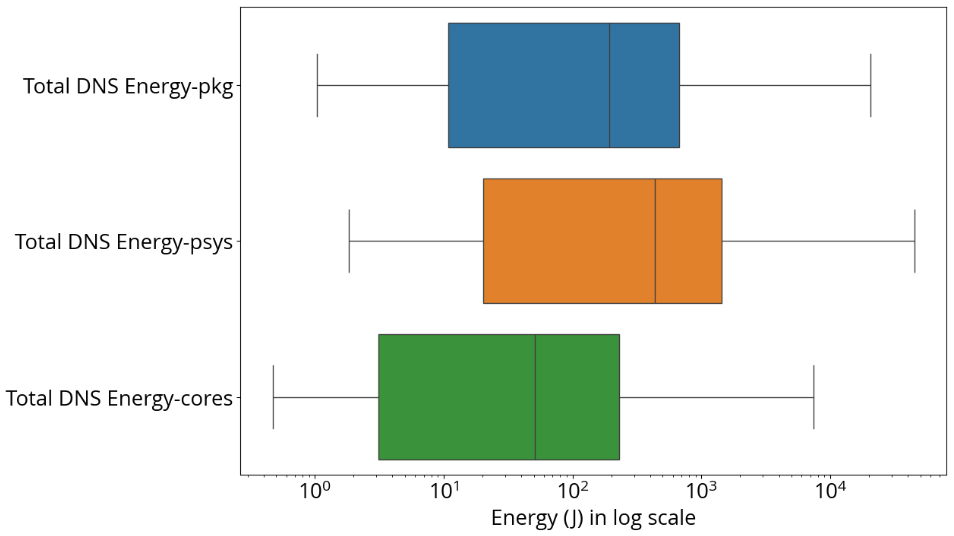
\includegraphics[width=1\linewidth]{images/energy.png}
    \caption{This box plot shows the energy (J) (in log scale) consumed in the DNS resolution of every domain required to load a page, for the 1000 websites we tested.}
    \label{fig:dns-energy}
\end{figure}

\section{Measuring Protocol Inefficiencies}
\label{Measuring Protocol Inefficiencies}
The DNS protocol and its implementation exhibit several inefficiencies. We performed several experiments which led us to the conclusion that the DNS protocol must be tweaked based on patterns observed in the requests for domain name resolution. We collected the list of the top 1000 domains from Cloudflare \cite{cloudflare}. We then explored several tools but weren't satisfied with the depth of analysis that they allowed for. Hence, we chose to build and develop our own scripts to analyze the DNS protocol. 

\subsection{Capturing Packets}
After getting the top 1000 domains, we built a sandboxed environment using Docker containers to simulate the page load of these top 1000 domains and capture the packets. This was necessary as we didn't want any other network traffic flowing through the same interface to interfere with our experiments. We also kept a timeout of 10 seconds to prevent being stuck on domains unaccessible through the NKN network. Furthermore, we took extra care to make sure that the DNS data we received was not cached and queries took the complete route through the resolvers. After going through the GNU manual for wget \cite{wget}, we concluded that running the following command in a docker container will do the trick. wget --no-dns-cache --no-verbose --timeout 10 -t 1 -c -E -H -k -K -p domain

\subsection{Analyzing the Captured Packets}
We developed several python scripts to analyze the captured packets. These scripts can be found in our \href{https://github.com/SachinJalan/DNS-Renaissance}{Github repository}. By leveraging tools like perf and dig (with special care not to use cached records) we collected the following information from the captured packets:
\begin{itemize}
    \item \textbf{Total Packets}: The total number of packets captured.
    \item \textbf{Total Bytes}: The total bytes of data exchanged.
    \item \textbf{Total DNS Packets}: The total number of DNS-specific packets.
    \item \textbf{Total DNS Bytes}: The total bytes of DNS-related traffic.
    \item \textbf{Total Time}: The total duration for complete page load.
    \item \textbf{Total DNS Time}: The total duration for DNS resolution.
    \item \textbf{Time to First Byte (TTFB)}: The time taken to receive the first byte of the response.
    \item \textbf{Total DNS Cycles}: The number of CPU cycles used during DNS resolution using the \texttt{perf} tool.
    \item \textbf{Total DNS Energy}: The energy consumption during DNS resolution, captured using the \texttt{perf} tool.
    \item \textbf{Visited Domains}: A list of all the domains involved in the page load with their respective record types.
\end{itemize}
These captured parameters were then analyzed and plotted.

\subsection{Analysis and Plots}
We first analyzed the packets that were involved in loading the complete page. We noticed that for the resolution of a single domain, various other domains were also queried for. For example, loading iitgn.ac.in required loading fonts.googleapis.com, googletagemanager, cdn.usefathom.com, www.facebook.com, and many more other than iitgn.ac.in. Figure \ref{fig:n_visited-domains} shows that a significant number of websites required multiple domain names to be resolved. Furthermore, we also noticed that a single domain was repeatedly queried multiple times throughout the average page load packet capture.

\begin{figure}[htbp]
    \centering
    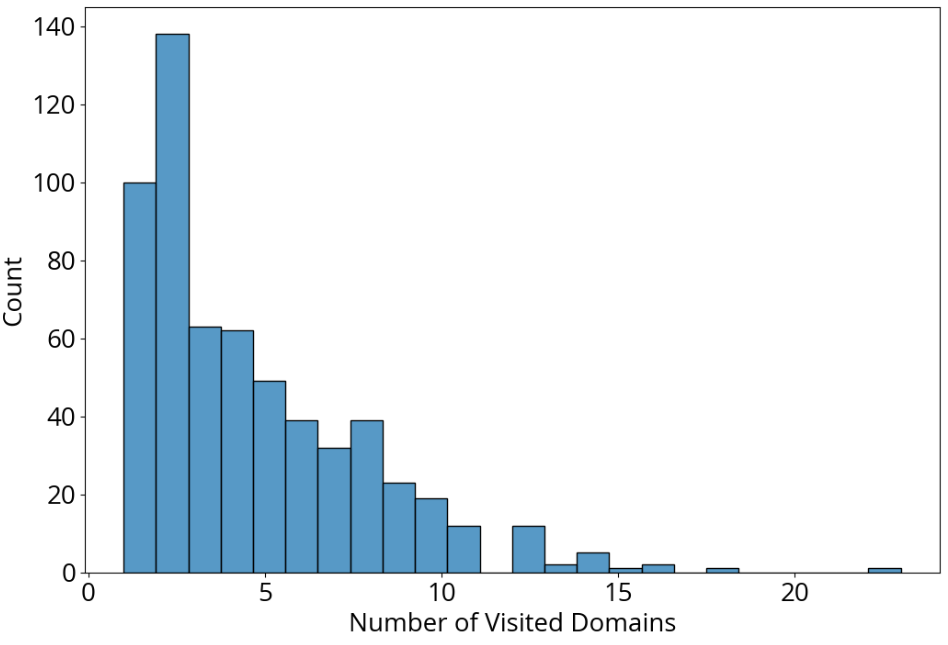
\includegraphics[width=1\linewidth]{images/n_visited-domains.png}
    \caption{This histogram shows the count of websites (out of 1000) vs the number of distinct domains visited.}
    \label{fig:n_visited-domains}
\end{figure}

Another heuristic we observed was that when an A record was queried, an AAAA query also accompanied in most cases. Figure \ref{fig:qtypes} shows this. 

\begin{figure}[htbp]
    \centering
    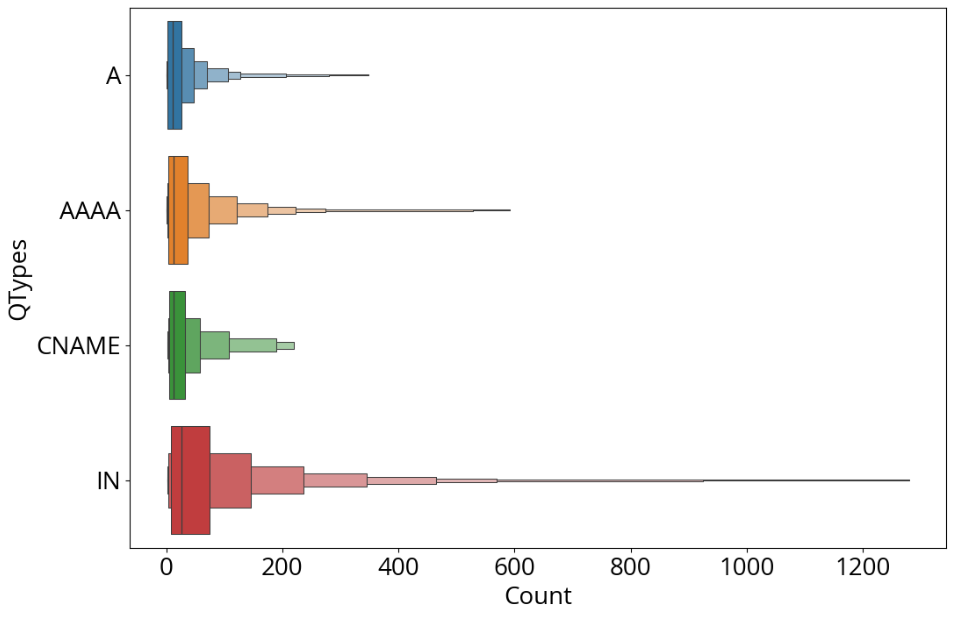
\includegraphics[width=1\linewidth]{images/qtypes.png}
    \caption{This boxen plot shows counts of the qtypes encountered in the page load of the top 1000 websites. Note how only A, AAAA, and CNAME were the record types that were requested for.}
    \label{fig:qtypes}
\end{figure}

Furthermore, we noticed that in one DNS query packet, only a single question was sent. However, the protocol allowed for multiple questions. This and the above-mentioned observations caused the DNS resolution to take a significant amount of time, packets, and bytes of the total page load. Figures \ref{fig:bytes-time-packets} shows this overhead caused by the current deployment of the DNS protocol. Figures \ref{fig:time-ratio}, \ref{fig:packet-ratio} and \ref{fig:bytes-ratio} are also provided for reference.

\begin{figure}[htbp]
    \centering
    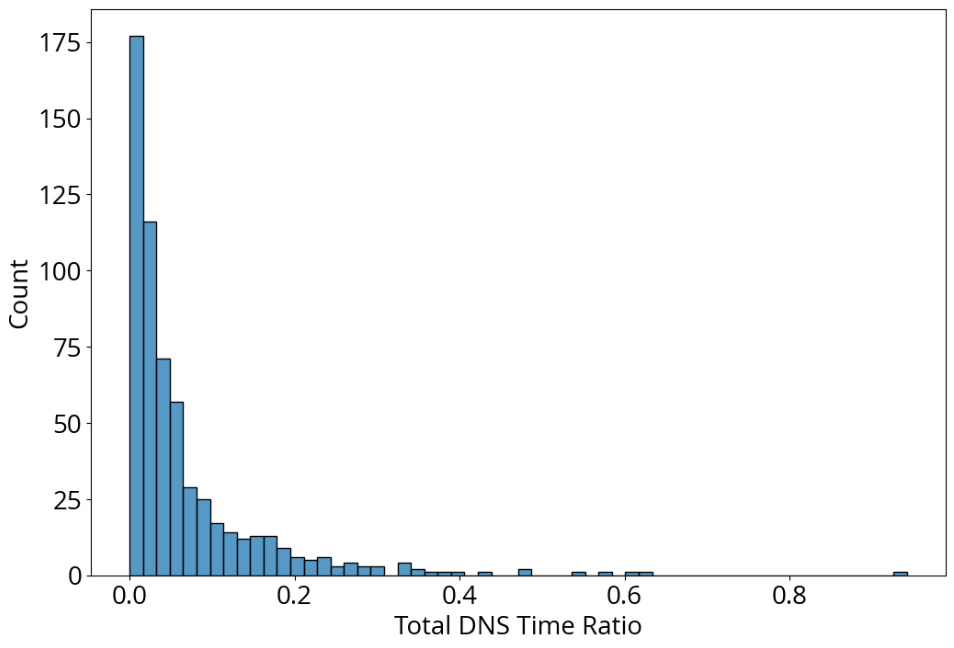
\includegraphics[width=1\linewidth]{images/time-ratio.png}
    \caption{This box plot shows the counts of the domains vs the ratio of time spent in DNS resolution to total page load time.}
    \label{fig:time-ratio}
\end{figure}

\begin{figure}[htbp]
    \centering
    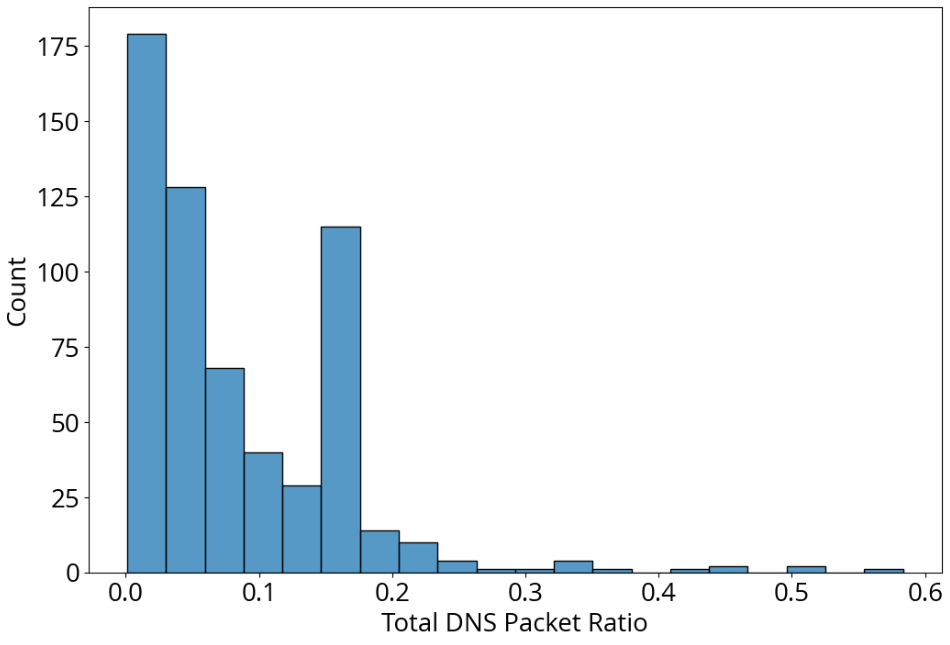
\includegraphics[width=1\linewidth]{images/packet-ratio.png}
    \caption{This box plot shows the counts of the domains vs the ratio of packets spent in DNS resolution to total packets for loading the complete page.}
    \label{fig:packet-ratio}
\end{figure}

\begin{figure}[htbp]
    \centering
    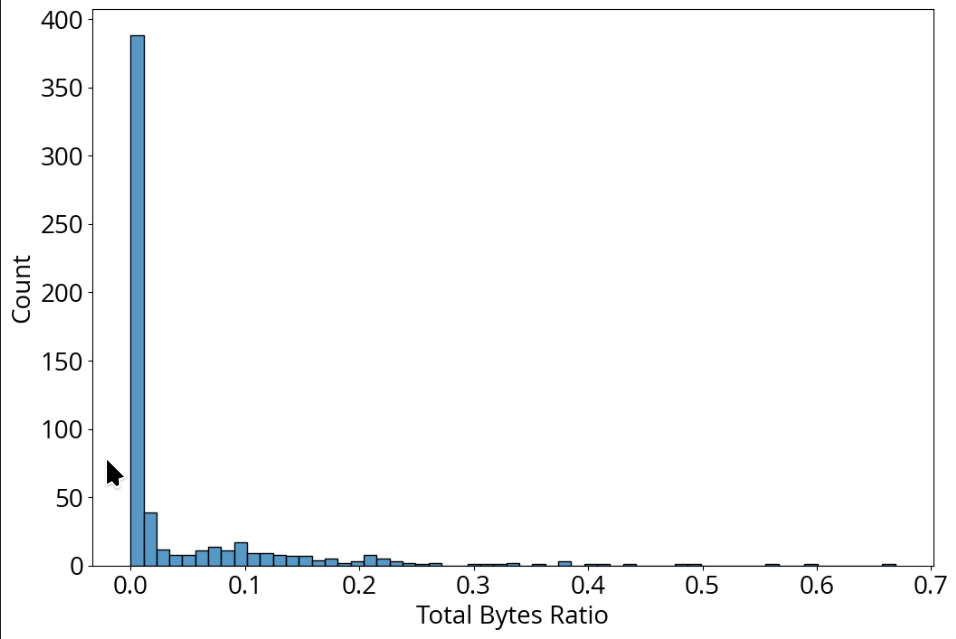
\includegraphics[width=1\linewidth]{images/bytes-ratio.png}
    \caption{This box plot shows the counts of the domains vs the ratio of bytes spent in DNS resolution to total bytes through the network to load the page.}
    \label{fig:bytes-ratio}
\end{figure}

\begin{figure}[htbp]
    \centering
    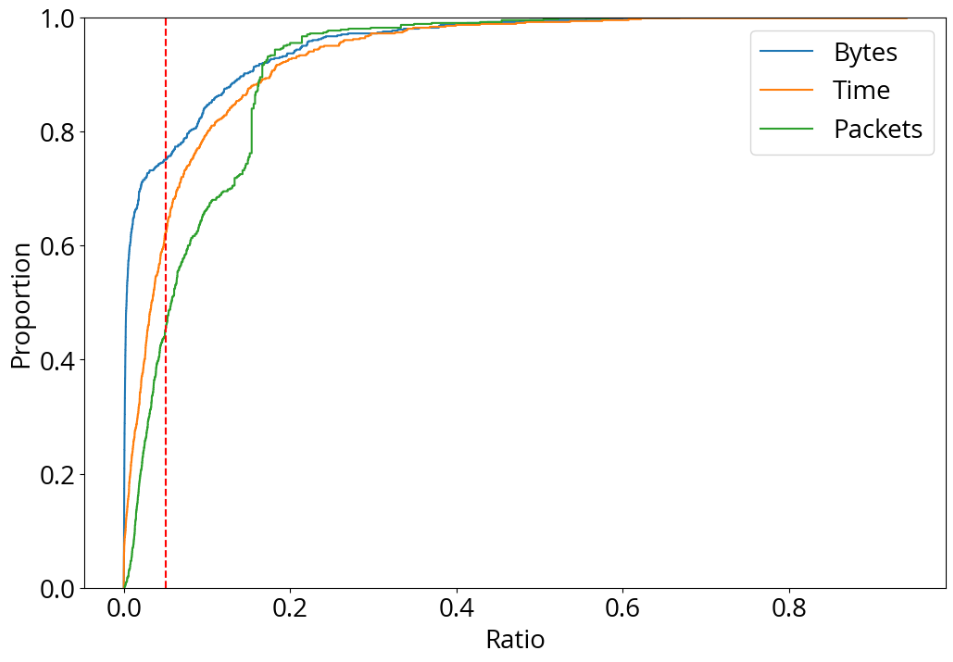
\includegraphics[width=1\linewidth]{images/bytes-time-packets.png}
    \caption{This is the CDF of the ratio of byte, time taken, and packets involved in DNS resolution. The 5\% critical region is also marked through a dashed red vertical line. From this, we infer
    that 60\%, 40\%, and 35\% of websites are beyond the
    5\% limit for bytes, time and packets taken respectively.}
    \label{fig:bytes-time-packets}
\end{figure}

We also observed that almost 7 bytes corresponding to the aa, z qdcount, nscount, arcount fields in the DNS header were never used in the page load of the top 1000 websites. We also noted that shift of transport layer protocol from UDP to TCP were very rare. It occurred 0.3\% out of the total 17277 DNS queries. These were mostly for AAAA records. This tells us that the DNS packets are small enough to fit into one UDP dataframe. Switching to TCP is rare, but when it occurs, we see about 1.2x increase in DNS resolution times.

Furthermore, we also checked if using a delegation like resolution other than the supported recursive and iterative would work in reducing the DNS resolution times. Delegation mode is where the name server is delegated the responsibility to respond back to the client with the record the client requested for. Since delegated mode is not supported natively by DNS, we measured it by calculating the time for resolving recursively ($RTT_r$), and the ping time to the name server ($RTT_p$) and finally calculating the delegation time ($RTT_d$) as $RTT_d = \frac{1}{2}RTT_r + \frac{1}{2}RTT_p$. However, delegated mode though theoretically involved less DNS packets, didn't provide much benefit as seen in figure \ref{fig:delegation} where only 5\% of the DNS requests encountered benefited from delegating the name server to return the answer to the client. This is because measuring the exact time for the resolution regardless of the modes is inaccurate. Moreover, this case arises when the path from name server to requester chosen was not the shortest.

\begin{figure}[htbp]
    \centering
    \begin{subfigure}[b]{1\linewidth}
        \centering
        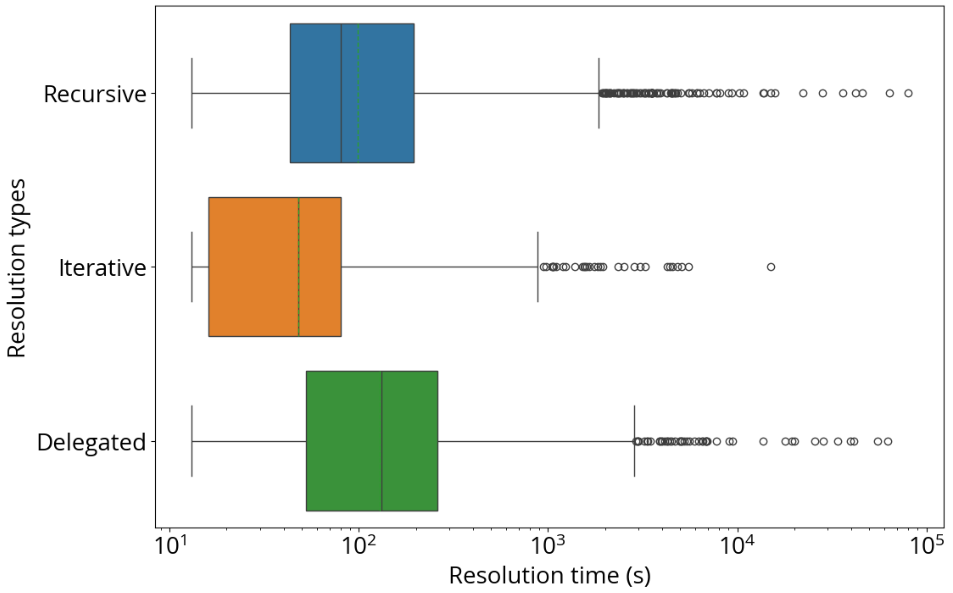
\includegraphics[width=\linewidth]{images/delegation-box.png}
        \caption{}
    \end{subfigure}
    \begin{subfigure}[b]{1\linewidth}
        \centering
        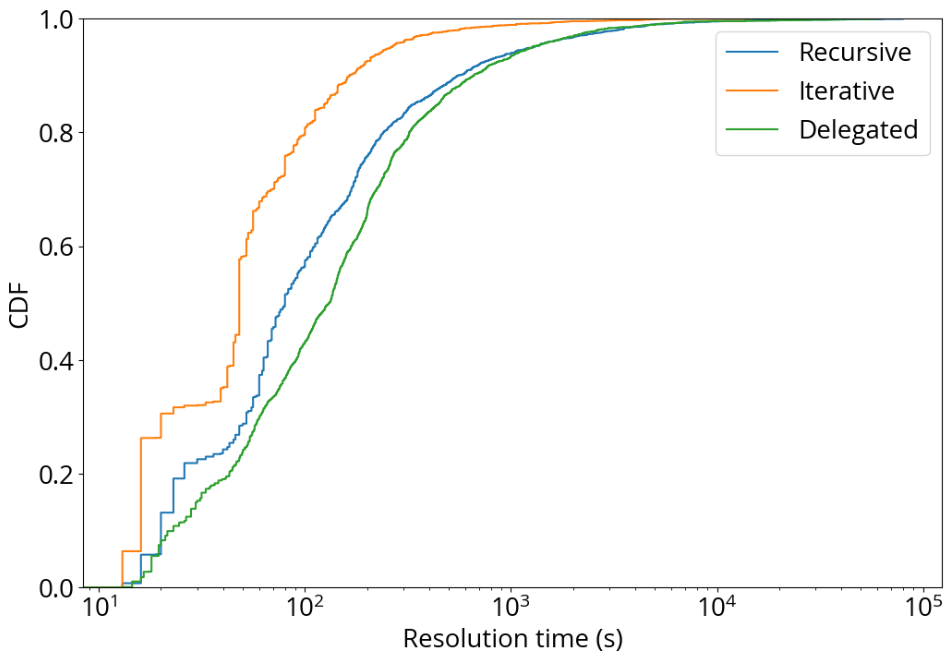
\includegraphics[width=\linewidth]{images/delegation-cdf.png}
        \caption{}
    \end{subfigure}
    \caption{The box plots (a) and the cdf plots (b) show a comparison between the resolution time taken while using recursive, iterated or delegated modes respectively.}
    \label{fig:delegation}
\end{figure}

With all this analysis, we had enough context set to proceed further to design a new DNS protocol that will address all these inefficiencies.

\section{Addressing the Problems: NDN-DNS}
We provide a solution that integrates the principles of Named Data Networking (NDN) to establish the foundations of a novel protocol for DNS resolution.

\subsection{Introduction to NDN}
Named Data Networking (NDN) is a transformative networking paradigm that redefines how information is requested, delivered, and secured across networks. Unlike traditional IP-based networking, which relies on identifying communication endpoints through IP addresses, NDN centers communication around the data itself, identified by human-readable, hierarchical names. This shift from host-based to data-based networking offers several advantages, including enhanced security, efficient content distribution, and in-network caching. Figure \ref{fig:ip-ndn-comp} illustrates the contrasting hourglass models of IP and NDN protocols.

\begin{figure}[htbp]
    \centering
    \includegraphics[width=1\linewidth]{images/ip-ndn-comp.png}
    \caption{Comparing IP and NDN protocol hourglasses \cite{ndn}}
    \label{fig:ip-ndn-comp}
\end{figure}

Key Principles of NDN are:
\begin{itemize}
    \item \textbf{Data-Centric Communication:} In NDN, communication is initiated by requesting specific data using its name rather than addressing a particular host. For instance, instead of contacting a server at an IP address (e.g., \texttt{192.168.1.1}) to retrieve a file, a user would directly request data by its name, such as \texttt{/example/education/file1}.
    \item \textbf{Named Data:} Every piece of data in NDN is uniquely identified by a hierarchical name that reflects its content and context. This structure facilitates efficient data organization, discovery, and routing. Please refer to figure \ref{fig:ndn-overview} where we see that the data consumer is simply requesting for the data by its name through the interest packet.
    \item \textbf{In-Network Caching:} NDN enables intermediate network nodes to store and cache data locally as it is transmitted. This in-network caching improves data retrieval efficiency, reduces latency, and minimizes redundant data transmissions by serving repeated requests directly from cache.
    \item \textbf{Content Security:} Unlike IP-based systems where security is often tied to endpoints, NDN integrates security directly into the data. Each piece of content is cryptographically signed, ensuring authenticity and integrity regardless of its storage or delivery path. From figure \ref{fig:ndn-overview} we can see that the data producer is signing the data packet before sending it to the consumer. Moreover a trusted web (refer figure \ref{fig:trusted-web}) is also formed making it difficult for an attacker to perform malicious activities.
\end{itemize}

\begin{figure}[htbp]
    \centering
    \includegraphics[width=1\linewidth]{images/ndn-overview.png}
    \caption{In an NDN network, one Interest packet can fetch one Data packet back from either the original data producer, or a router cache, or from a dedicated data repository\cite{ndn}}
    \label{fig:ndn-overview}
\end{figure}

\begin{figure}[htbp]
    \centering
    \includegraphics[width=1\linewidth]{images/trusted-web.png}
    \caption{A rich web of trustworthy information arises from named, signed data. Attacker’s job increases exponentially. This is because the signature in a sense is a pointer to a content an so on. \cite{ndn-presentation}}
    \label{fig:trusted-web}
\end{figure}

NDN offers several advantages over traditional IP-based networking. Also treating DNS records as named content, we can leverage NDN's inherent benefits to redefine DNS resolution. Thus we propose the following NDN-DNS protocol.

\subsection{NDN-DNS Protocol Overview}
In our approach, DNS queries and responses are expressed using NDN principles. Each DNS record type (e.g., A, AAAA, MX) is treated as named content (with the name being the domain name), allowing the retrieval of records directly by their hierarchical domain names. This means that all the records corresponding to a single domain is a single content, all signed by the name server (producer). This approach redefines DNS resolution to leverage NDN’s inherent benefits, such as in-network caching, efficient data retrieval, and enhanced security through cryptographic signing of content.

We claim that this solution that we provide easily addresses the inefficiencies of the existing DNS protocol that we have previously outlined. The benefits of NDN-DNS are:
\begin{itemize}
    \item All record types of a particular domain can be in a single content packet. Thus when an application requests for a particular record type we can provide all the record types knowing that the application will ask the other record types too. This concept is illustrated in figure \ref{fig:dns-content}. This negates the need for multiple queries for the different records of the domain. This will reduce the time taken to load the page completely.
    \item Nodes that are performing DNS queries can very well benefit from the caching of the contents in the path. Figure \ref{fig:caching-benefit} shows how if someone from IITGN queries for a domain that someone from GIFT City has already queried for, the response can be found in the cache of GIFT City. This reduces the resolution time because we will not be going to the Internet to get the response.
    \item We can ensure that the records reach the requester from the shortest possible path. This is because the routers in the path can cache the content and respond to the requester. This is shown in figure \ref{fig:caching-benefit}.
    \item Security is handled appropriately as each content is signed by the producer in NDN. In our case the Name Server (the producer) can sign the content of the records it produces. Security is implemented as a trusted web as seen in figure \ref{fig:trusted-web}
\end{itemize}

\begin{figure}[htbp]
    \centering
    \includegraphics[width=1\linewidth,trim={0 15cm 0 0.4cm},clip]{images/dns-content.pdf}
    \caption{In NDN-DNS, all record types of a domain are treated as a single content packet, allowing efficient retrieval of all records in a single query. Notice how the response can come from router in the path other than the producer due to caching. The dotted lines represent the RTT that was saved due to caching.} 
    \label{fig:dns-content}
\end{figure}

\begin{figure}[htbp]
    \centering
    \includegraphics[width=1\linewidth,trim={0 13cm 0 0.4cm},clip]{images/caching-benefit.pdf}
    \caption{This figure shows how the caching of the content in the path can benefit the resolution time on a global scale. The response can be found in the cache of GIFT City if someone from IITGN queries for a domain that someone from GIFT City has already queried for.}
    \label{fig:caching-benefit}
\end{figure}

\subsection{Analysis of Proposed Solution}
We verified the benefits of the proposed NDN-DNS protocol and quantified them using the ICARUS-ICN Simulator \cite{icarus-simutools14}.
\subsubsection{Introduction to ICARUS-ICN Simulator \cite{icarus-simutools14}} Icarus is a Python-based discrete-event simulator for evaluating caching performance in Information Centric Networks (ICN) that models the behavior of NDN networks, allowing researchers to analyze the performance of NDN-based applications and protocols. We configured the simulator to simulate the behavior of DNS resolution using NDN-DNS and compared it with traditional DNS resolution. A few parameters that we used in the simulation are:
\begin{itemize}
    \item \textbf{Cache Size:} The size of the cache in each router in the network. Greater cache size means more content can be stored in the cache. The cache size is measured in terms of the number of contents that can be stored, hence we assume that the size of DNS records for all the domains is the same.
    \item \textbf{Network Topology:} The structure of the network, including the number of routers and their interconnections. The sources and the producers. The cacheable routers are called ICR candidates.
    \item \textbf{Workload:} This is the pattern of requests that the sources will do in the network topology.
    \item \textbf{$\alpha$ Content Distribution:} This parameter governs the distribution of contents in the requests by the sources. A request that a source makes is sampled from a zipf distribution with parameter $\alpha$. The higher the alpha, the more skewed the distribution is meaning that the sources are requesting for the same content and the cache can be utilized more effectively. 
    \item \textbf{Network Request Rate:} This represents Number of requests per second (over the whole network).
    \item \textbf{Warmup Requests}: These are the number of content requests that are made to prepopulate the caches.
    \item \textbf{Measured Requests}: These are the number of content requests that are made to measure the performance of the network.
    \item \textbf{Caching Strategy:} The caching strategy that the routers will use to cache the content. We used the LRU caching strategy. Various caching strategies like LCD, LCE, random, random-bernoulli, etc. can be used.
    \item \textbf{Cache Policy:} This is the cache replacement policy that the caches will follow. We can choose one from LRU, RAND, FIFO and LFU.
\end{itemize}

\subsubsection{Results}
We designed our own workload compatible with ICARUS for both the existing DNS protocol and the proposed NDN-DNS protocol. This had to be done as we wanted to do an apple to apple comparison. Furthermore we changed the existing topologies like the GEANT 2012 topology and converted some of the sources into root servers, some into TLD servers and some into name servers. We also added special rules to ensure that each server provides content that it has to. We also assumed that each name server serves as a producer for just one domain. This implies that the number of contents in the network is the number of domains that is the number of name servers in the network. Scripts for these can be found in our fork of the ICARUS-ICN simulator \href{https://github.com/eelfire/icarus/tree/dnsr/examples/dnsr/config4}{here}. In the experiment we conducted, we used the GEANT 2012 topology. This had 13 sources in total out of which one was the root, one was the TLD and 11 were name servers. This means that there were only 11 domains. We used 10 warmup requests and 300 measured requests. We collected results for cache sizes of 0.1\%, 0.5\%, 1\%, 5\% and 10\% of the full network. However, we show only the results from cache size of and 1\% of the network. These results can be seen in figures and \ref{fig:icarus-c0.01}. We can clearly see that the proposed solution is better than the existing DNS protocol in terms of latency and this is exactly because of the benefit of caching.

\begin{figure}[htbp]
    \centering
    \begin{subfigure}[b]{\linewidth}
        \centering
        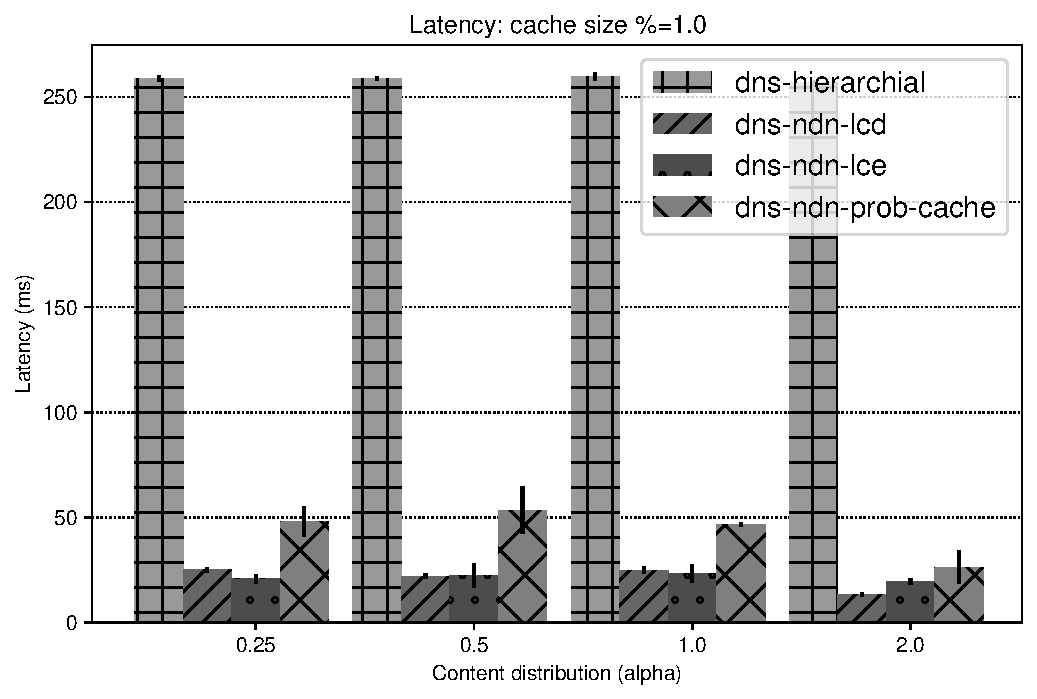
\includegraphics[width=0.85\linewidth]{images/LATENCY_C=0.01.pdf}
        \caption{Latency vs alpha (cache size 1\%) for the existing DNS protocol (dns-hierarchical) and the proposed NDN-DNS protocol (dns-ndn-*) on some caching strategies. Here latency means complete time for the resolution of the domain. That is time taken for root and TLD servers to respond back to the source are also included in case of dns-hierarchical.}
    \end{subfigure}
    \begin{subfigure}[b]{\linewidth}
        \centering
        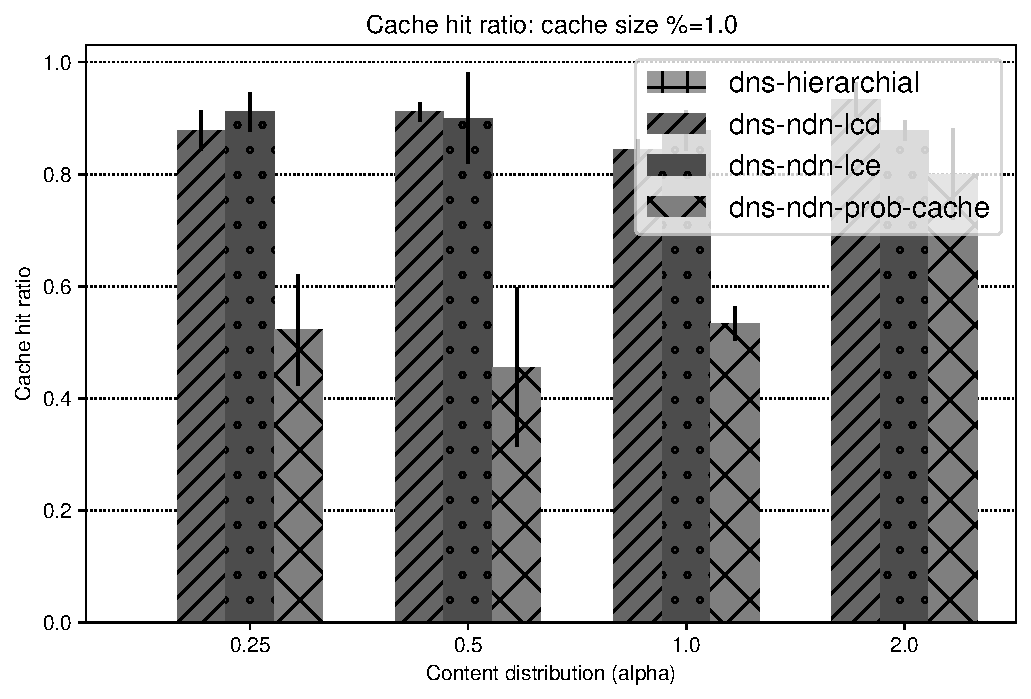
\includegraphics[width=0.85\linewidth]{images/CACHE_HIT_RATIO__C=0.01.pdf}
        \caption{Cache hit ratio vs alpha (cache size 1\%) for the existing DNS protocol and the proposed NDN-DNS protocol on some caching strategies.}
    \end{subfigure}
    \begin{subfigure}[b]{\linewidth}
        \centering
        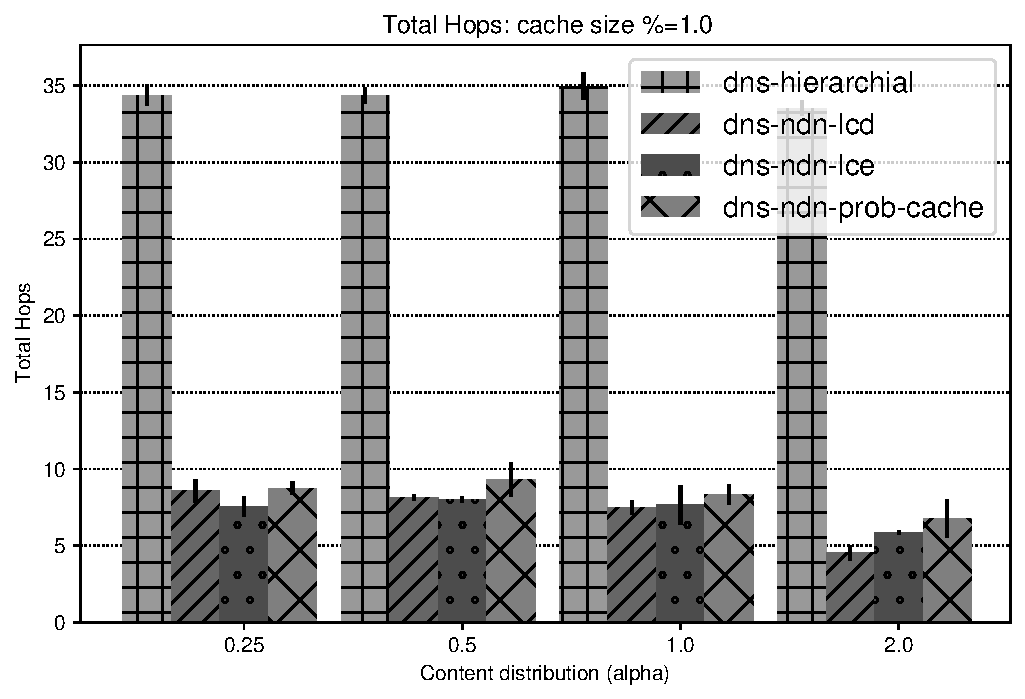
\includegraphics[width=0.85\linewidth]{images/TOTAL_HOPS_C=0.01.pdf}
        \caption{Total hops vs alpha (cache size 1\%) for the existing DNS protocol and the proposed NDN-DNS protocol on some caching strategies. Here the total hops referes to the number of hops the request took plus the number of hops the response took to reach the source.}
    \end{subfigure}
    \caption{From the measured latency, cache hit ratio and total hops, we can see that the proposed NDN-DNS protocol is better than the existing DNS protocol. The total hops is also lowest for the proposed NDN-DNS protocol. This and the cache hit ratio clearly show that the lower latency by ndn-dns comes from the caching.}
    \label{fig:icarus-c0.01}
\end{figure}

% \begin{figure}[htbp]
%     \centering
%     \begin{subfigure}[b]{\linewidth}
%         \centering
%         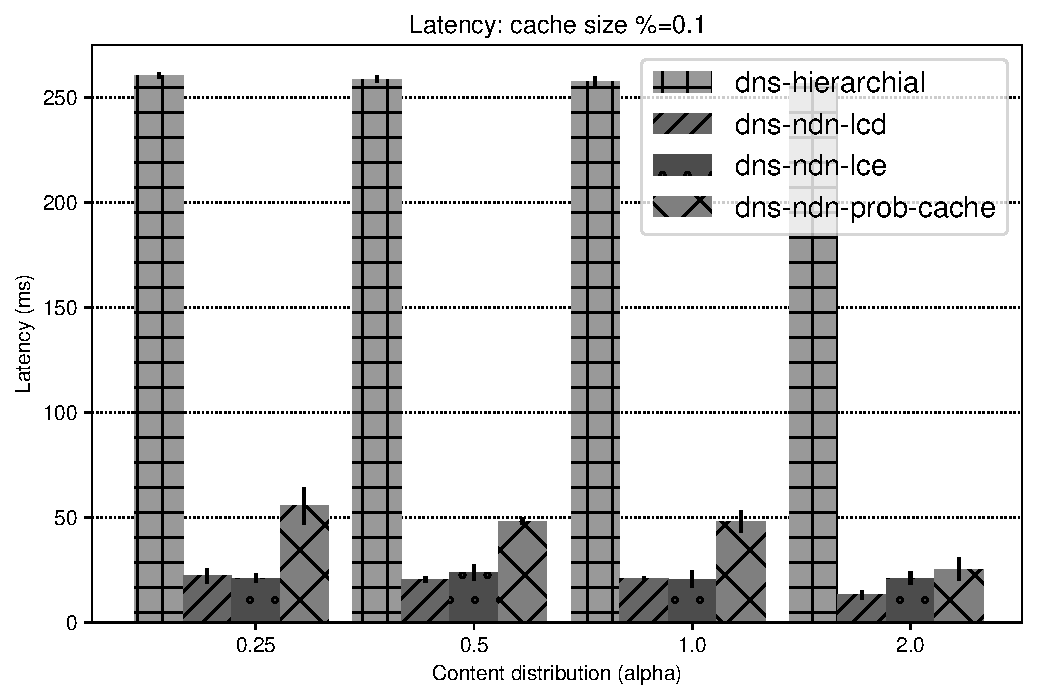
\includegraphics[width=0.9\linewidth]{images/LATENCY_C=0.001.pdf}
%         \caption{Latency vs alpha (cache size 0.1\%) for the existing DNS protocol (dns-hierarchical) and the proposed NDN-DNS protocol (dns-ndn-*) on some caching strategies. Here latency means complete time for the resolution of the domain. That is time taken for root and TLD servers to respond back to the source are also included in case of dns-hierarchical.}
%     \end{subfigure}
%     \begin{subfigure}[b]{\linewidth}
%         \centering
%         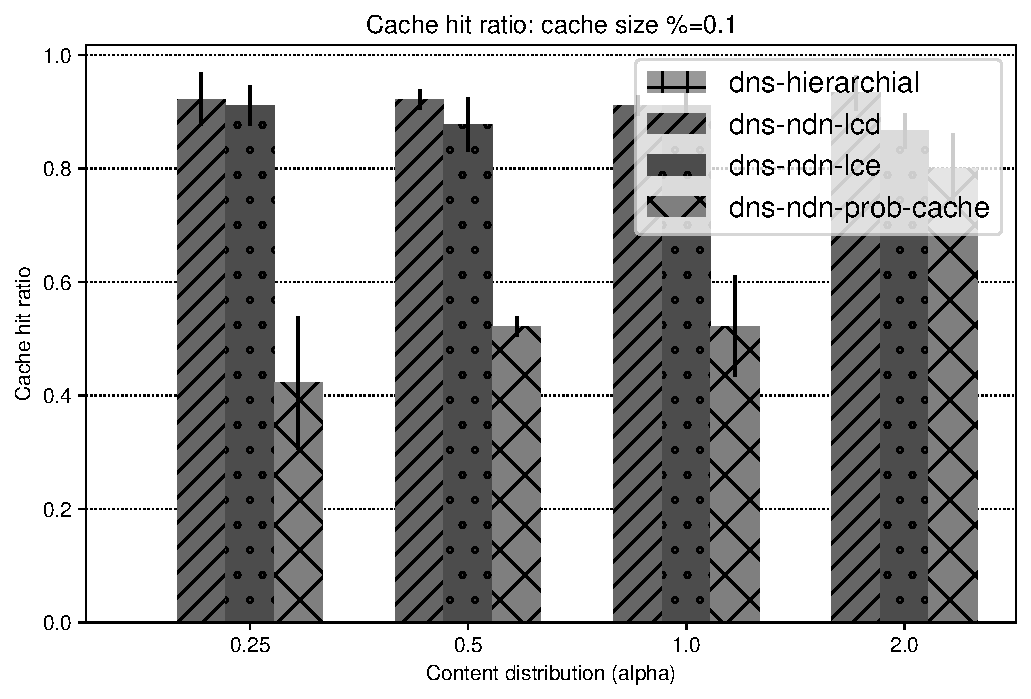
\includegraphics[width=0.9\linewidth]{images/CACHE_HIT_RATIO__C=0.001.pdf}
%         \caption{Total hops vs alpha (cache size 0.1\%) for the existing DNS protocol and the proposed NDN-DNS protocol on some caching strategies. Here the total hops referes to the number of hops the request took plus the number of hops the response took to reach the source.}
%     \end{subfigure}
%     \begin{subfigure}[b]{\linewidth}
%         \centering
%         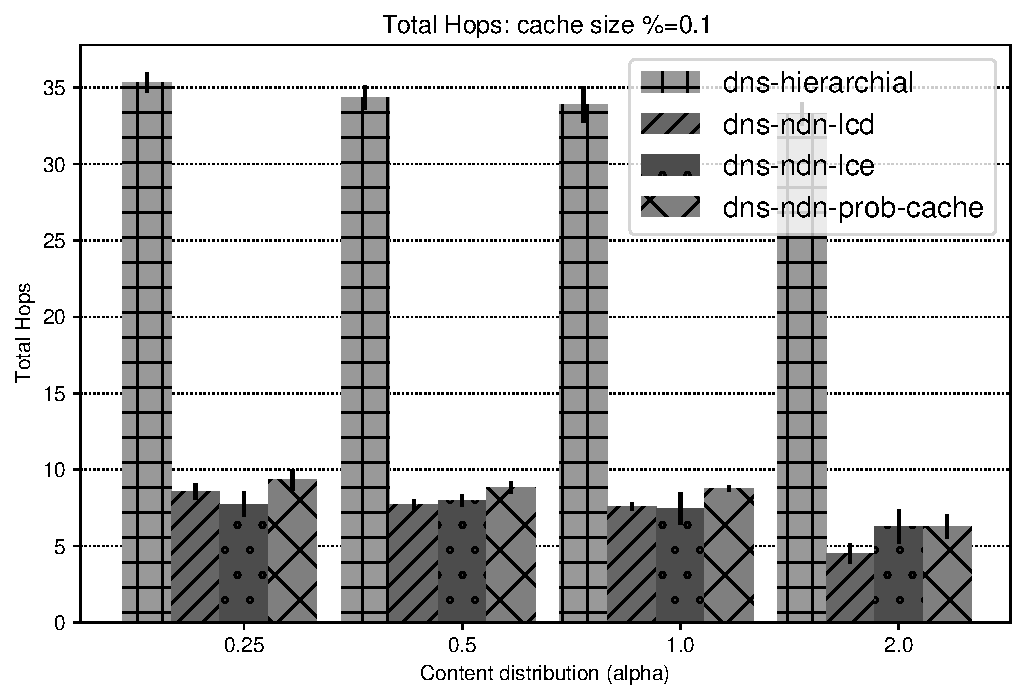
\includegraphics[width=0.9\linewidth]{images/TOTAL_HOPS_C=0.001.pdf}
%         \caption{Total hops vs alpha (cache size 0.1\%) for the existing DNS protocol and the proposed NDN-DNS protocol on some caching strategies. Here the total hops referes to the number of hops the request took plus the number of hops the response took to reach the source.}
%     \end{subfigure}
%     \caption{Similar observations as made in figure \ref{fig:icarus-c0.01} can be made here.}
%     \label{fig:icarus-c0.001}
% \end{figure}

\section{Related Works}
Several works have explored the inefficiencies of the traditional DNS protocol and proposed various solutions to address these issues. For instance, the work by Mockapetris and Dunlap \cite{mockapetris1983dns} laid the foundation for DNS, highlighting its scalability and robustness. However, subsequent studies, such as those by Arends et al. \cite{rfc4033}, identified security vulnerabilities in DNS, leading to the development of DNS-SEC. Despite its security enhancements, DNS-SEC's complexity and computational overhead have been well-documented by researchers like Atkins and Austein \cite{rfc3833}.

In the context of IoT and edge devices, the limitations of traditional DNS have been further emphasized. The work titeld, "The DNS in IoT: Opportunities, Risks, and Challenges" \cite{dns-iot} have explored lightweight security solutions for DNS in IoT environments. Additionally, the concept of Named Data Networking (NDN) has been proposed as a promising alternative to traditional IP-based networking. Jacobson et al. \cite{jacobson2009networking} introduced NDN, highlighting its potential for efficient content distribution and enhanced security.

Woeks by Raza et al. \cite{dns-dele} have explored annd tested sending an authoritative response from a non-authoritative DNS server. They observerd a 2x drop in resolution time. This further strengthens our intuition for a delegated model that is inbuilt into the NDN-DNS solution.

Our proposed NDN-DNS protocol builds on these foundational works, leveraging the principles of NDN to address the inefficiencies of traditional DNS. By treating DNS records as named content and utilizing in-network caching, our approach aims to improve the efficiency and security of DNS resolution, particularly in resource-constrained environments.

\section{Conclusion}
In this report, we have highlighted the inefficiencies of the traditional DNS protocol, particularly in the context of IoT and edge devices. Through extensive experiments and analysis, we identified key pain points in the current DNS implementation, including high computational overhead, increased latency, and security vulnerabilities. To address these issues, we proposed a novel DNS protocol based on Named Data Networking (NDN).

Our NDN-DNS protocol leverages the principles of NDN, treating DNS records as named content and utilizing in-network caching to improve efficiency and security. We validated our approach using the ICARUS-ICN simulator, demonstrating significant improvements in latency and cache hit ratios compared to traditional DNS.

Future work will focus on further optimizing the NDN-DNS protocol and exploring its deployment in real-world IoT and edge environments. We believe that our proposed solution has the potential to significantly enhance the performance and security of DNS resolution, paving the way for more efficient and secure Internet communication.

\bibliographystyle{plain}
\bibliography{references}
\end{document}
